\documentclass[]{article}

% Use utf-8 encoding for foreign characters
\usepackage[latin1]{inputenc}


% Setup for fullpage use
\usepackage{fullpage}
% Uncomment some of the following if you use the features
%
% Running Headers and footers
%\usepackage{fancyhdr}

% Multipart figures ´¡009753º
% More symbols
%\usepackage{amsmath}\emph{}
%\usepackage{amssymb}
%\usepackage{latexsym}

% Surround parts of graphics with box
\usepackage{boxedminipage}

% Package for including code in the document
\usepackage{listings}

% Package for subfigure
\usepackage{graphicx}


% If you want to generate a toc for each chapter (use with book)
\usepackage{minitoc}

% This is now the recommended way for checking for PDFLaTeX:
\usepackage{ifpdf}
%\newif\ifpdf
%\ifx\pdfoutput\undefined
%\pdffalse % we are not running PDFLaTeX
%\else
%\pdfoutput=1 % we are running PDFLaTeX
%\pdftrue
%\  XCM CNXKJBWQGFUHREPUYT485¨94-32¨1fi
\usepackage[all,light]{draftcopy}
%\draftcopyName{PROBABILIDAD II}{5}


\usepackage{amsmath}
\usepackage{amsfonts}
\usepackage{bm}
\usepackage{layout}
\usepackage{fancyhdr}
\pagestyle{fancy}
%\ifpdf
%\usepackage[pdftex]{graphicx}
%\else
%\usepackage{graphicx}
%\fi
\usepackage[top=2cm,bottom=3cm,headsep=1.5cm]{geometry}
\usepackage{hyperref}
\newcommand{\R}{\mbox{$I\!\!R$}}
\usepackage{cleveref}

\begin{document}

\lhead{\textsf{UCSC - Fall 2016} \\{AMS 374}}
\chead{\Large{General Linear Model}}
\rhead{\textsf{Student:} \\{Rui Meng}}
\renewcommand{\headrulewidth}{0.4pt}
\renewcommand{\footrulewidth}{0.4pt}


\begin{center}
\section*{\underline{Homework 2}}
\end{center}

\begin{enumerate}  \Large{

\item (Ex. 1)
Let $y_i$ be realizations of independent random variables $Y_i$ with Poisson($\mu_i$) distributions, where $E(Y_i) = \mu_i$ for $i = 1,\ldots,n$.
\begin{itemize}
	\item[(a)] Obtain the expression fro the deviance for comparison of the full model, which assumes a different $\mu_i$ for each $y_i$, with a reduced model defined by a Poisson GLM with link function $g(\cdot)$. That is, under the reduced model, $g(\mu_i) = \eta_i = \bm{x}_i^T \bm{\beta}$, where $\bm{\beta} = (\beta_1,\ldots,\beta_p)^T$ (with $p<n$) is the vector of regression coefficients corresponding to covariates $\bm{x}_i = (x_{i1},\ldots,x_{ip})^T$ 
	\item[(b)] Show the expression for the deviance simplifies to $2\sum_{i=1}^{n}y_i\log(y_i/\hat{\mu}_i)$, for the special case of the reduced model in part (a) with $g(\mu_i) = \log(\mu_i)$, and linear predictor that includes an intercept, that is, $\eta_i = \beta_1 + \sum_{j=2}^{p}x_{ij}\beta_j$, for $i = 1,\ldots,n$.
\end{itemize}

\item[Sol. 1]
\begin{itemize}
	\item[(a)] Since $Y_i$ follows the Poisson ($\mu_i$) distributions, let $y_i|\mu_i\stackrel{iid}{\sim}\frac{\mu_i^{y_i} e^{-\mu_i}}{y_i!}$.
	Then the log-likelihood function can be expressed as
	\begin{eqnarray}
	\ell(\hat{\bm{\mu}};\bm{y}) & = & \sum_{i = 1}^{n} \ell(\hat{\mu_i},y_i)\\
	& = & \sum_{i = 1}^{n} e^{y_i\ln \mu_i - \mu_i - \ln y_i!}\\
	\end{eqnarray}
	which shows that the nature parameter $\theta_i = \ln\mu_i$ and $b(\theta) = e^\theta$. And then $\mu_i = e^{\theta_i}$.\\
	Next, substituting $\mu_i$ with $\theta_i$, we have $\ell(\hat{\bm{\theta}};\bm{y}) = \sum_{i=1}^{n}y_i\theta_i-e^\theta_i-\ln y_i!$\\
	The deviance for Poisson GLM should be
	\begin{eqnarray}
	D & = & -2(\ell(\hat{\bm{\theta}};\bm{y})-\ell(\tilde{\bm{\theta}};\bm{y})) \\
	& = & -2\sum_{i = 1}^{n}[y_i(\hat{\theta_i}-\tilde{\theta_i})-e^{\hat{\theta}_i}+e^{\tilde{\theta}_i}]\\
	& = & -2\sum_{i = 1}^{n}[y_i\ln\frac{\hat{\mu_i}}{\tilde{\mu_i}}-\hat{\mu_i}+\tilde{\mu_i}]
	\end{eqnarray}
	Since the full model implies that $\tilde{\mu}_i = y_i$, substituting the equation to the expression above generates that 
	\begin{equation}
	D = 2\sum_{i=1}^{n}[y_i\ln\frac{y_i}{\hat{\mu}_i}-(y_i-\hat{\mu}_i)].
	\end{equation}
	\item[(b)] If $g(\mu_i) = \ln(\mu_i)$ and $\eta_i = \bm{\beta}^T\bm{x}_i$, because $\hat{\beta}$ maximizes $\ell(\hat{\bm{\theta}};\bm{y})$, we have $\frac{\partial\ell(\bm{\theta};\bm{y})}{\partial\bm{\beta}} = \bm{0}$. Because 
	\begin{eqnarray}
	\frac{\partial\ell}{\partial\beta_j} & = & \sum_{i = 1}^{n}\frac{\partial\ell}{\partial\theta_i}\frac{\partial\theta_i}{\partial\mu_i}\frac{\partial\mu_i}{\partial\eta_i}\frac{\partial\eta_i}{\beta_j} \\
	& = & \sum_{i = 1}^{n}(y_i-e^{\theta_i})\mu_i^{-1}\mu_i x_{ij} \\
	& = & \sum_{i = 1}^{n}(y_i-\mu_i) x_{ij}
	\end{eqnarray}
	where $x_{i1} = 1$ for $i = 1,\ldots,n$. Because $\frac{\partial\ell}{\beta_1} = 0$, we derive that $\sum_{i = 1}^{n}(y_i-\hat{\mu_i}) x_{i1} = \sum_{i = 1}^{n}(y_i-\hat{\mu_i}) = 0$.\\
	Therefore, 
	\begin{eqnarray}
	D & = & 2\sum_{i=1}^{n}[y_i\ln\frac{y_i}{\hat{\mu}_i}-(y_i-\hat{\mu}_i)] \\
	& = & 2\sum_{i=1}^{n}y_i\ln\frac{y_i}{\hat{\mu}_i}
	\end{eqnarray}
\end{itemize}

\item (Ex. 2)
Let $y_i$, $i = 1,\ldots,n$ be realizations of independent random variables $Y_i$ following gamma($\mu_i,\nu$) distributions, with densities given by
\begin{equation*}
f(y_i|\mu_i,\nu) = \frac{(\nu/\mu_i)^\nu y_i^{\nu-1}\exp(-\nu y_i/\mu_i)}{\Gamma(\nu)}, y_i>0, \nu>0, \mu_i>0,
\end{equation*}
where $\Gamma(\nu) = \int_0^{\infty} t^{\nu-1}\exp(-t)dt$ is the Gamma function.
\begin{itemize}
	\item[(a)] Express the gamma distribution as a member of the exponential dispersion family.
	\item[(b)] Obtain the scaled deviance and deviance for the comparison of the full model, which includes a different $\mu_i$ for each $y_i$, with a gamma GLM based on link function $g(\mu_i) = \bm{x}_i^T\bm{\beta}$, where $\bm{\beta} = (\beta_1,\ldots,\beta_p)$ $(p<n)$is the vector of regression coefficients corresponding to a set of $p$ covariates.
\end{itemize}

\item[Sol. 2]
\begin{itemize}
	\item[(a)]  The density function can be rewritten as 
	\begin{eqnarray*}
	f(y_i|\mu_i,\nu) & = & \exp(\nu\ln(\frac{\nu}{\mu_i})+(\nu-1)\ln y_i -\frac{\nu}{\mu_i}y_i - \ln\Gamma(\nu))\\
	& = & \exp(\frac{\alpha_iy_i-\ln\frac{\alpha_i}{\theta}}{\theta} + (\frac{1}{\theta}-1)\ln y_i - \ln\Gamma(\frac{1}{\theta}))\\
	& = & \exp(\frac{\alpha_iy_i-\ln \alpha_i}{\theta} + \frac{\ln \theta}{\theta} + (\frac{1}{\theta}-1)\ln y_i - \ln\Gamma(\frac{1}{\theta}))
	\end{eqnarray*}
	where $\alpha_i = -\frac{1}{\mu_i}$ and $\theta = \frac{1}{\nu}$. It suggests that $\alpha_i$ is the nature parameter and $\theta$ is the disperse parameter and this distribution belongs to the exponential distribution family.
	\item[(b)] The scaled deviance and deviance are derived as follows:
	\begin{eqnarray}
	D^* & = & -2(\ell(\hat{\bm{\mu}},\nu;\bm{y}) - \ell(\tilde{\bm{\mu}},\nu;\bm{y})) \\
	& = & -2\sum_{i = 1}^{n}(\nu\ln(\frac{\tilde{\mu}_i}{\hat{\mu}_i}) - \frac{\nu y_i}{\hat{\mu}_i} + \frac{\nu y_i}{\tilde{\mu}_i}) \\
	& = & \nu \cdot -2\sum_{i = 1}^{n}(\ln \frac{\tilde{\mu}_i}{\hat{\mu}_i} - \frac{y_i}{\hat{\mu}_i} + \frac{y_i}{\tilde{\mu}_i})\\
	D & = &  -2\sum_{i = 1}^{n}(\ln \frac{\tilde{\mu}_i}{\hat{\mu}_i} - \frac{y_i}{\hat{\mu}_i} + \frac{y_i}{\tilde{\mu}_i})
	\end{eqnarray}
	Since $\tilde{\mu_i} = y_i$, we have that $D^* = \nu \cdot -2\sum_{i = 1}^{n}(\ln \frac{y_i}{\hat{\mu}_i} - \frac{y_i}{\hat{\mu}_i} + 1)$ and $D = -2\sum_{i = 1}^{n}(\ln \frac{y_i}{\hat{\mu}_i} - \frac{y_i}{\hat{\mu}_i} + 1)$, where $\hat{\mu}_i = g^{-1}(\bm{x}_i^T\hat{\bm{\beta}})$
\end{itemize}

\item (Ex. 3)
Consider the data set from:\\
http://www.stat.columbia.edu/~gelman/book/data/fabric.asc\\
on the incidence of faults in the manufacturing of rolls of fabrics. The first column contains the length of each roll (the covariate with values $x_i$), and the second contains the number of faults (the response with means $\mu_i$).
\begin{itemize}
	\item[(a)] Use R to fit a Poisson GLM, with logarithmic link,
	\begin{equation}
	\ln(\mu_i) = \beta_1 + \beta_2x_i
	\end{equation}
	to explain the number of faults in terms of length of roll.
	\item[(b)] Fit the regression model for the response means in (1) using the quasi-likelihood estimation method, which allows for a dispersion parameter in the response variance function. (Use the quasipoisson "family" in R.) Discuss the results.
	\item[(c)] Derive point estimates and asymptotic interval estimates for the linear predictor, $\eta_0 = \beta_1 + \beta_2x_0$, at a new value $x_0$ for length of roll, under the standard (likelihood) estimation method from part (a), and the quasi-likelihood estimation from part (b). Evaluate the point and interval estimates at $x_0 = 500$ and $x_0=995$. (Under both cases, use the asymptotic bivariate normality of $(\hat{\beta}_1,\hat{\beta}_2)$ to obtain the asymptotic distribution of $\hat{\eta}_0 = \hat{\beta}_1 + \hat{\beta}_2x_0$.)
\end{itemize}
\item[(Sol. 3)]
\begin{itemize}
	\item[(a)] After using R to fit a Poisson GLM, we have the results in Table~\ref{est}:
	\begin{table}
		\centering
		\caption{Estimation for a Poisson GLM}
		\begin{tabular}{|c|c|c|}
			\hline
			& estimate & std \\
			\hline
			$\beta_0$ & 1.04 & 0.21 \\
			\hline
			$\beta_1$ & 0.00 & 0.00 \\
			\hline
		\end{tabular}
		\label{est}
	\end{table}
	\item[(b)] The estimates of coefficients of covariates $\bm{\beta}$ are exactly same. And the disperse estimate is 2.24. This is because that the estimate of nature parameter which related to $\bm{\beta}$ is free of the disperse parameter $\sigma$. It suggests that the two methods should have the same nature parameter and so the same $\hat{\bm{\beta}}$.
	\item[(c)] According to the MLE property, under the regulation condition, $\hat{\bm{\beta}} \stackrel{\cdot}{\sim}\mathcal{N}(\bm\beta, J^{-1}(\hat{\bm{\beta}}))$. Considering the disperse parameter, $\hat{\bm{\beta}} \stackrel{\cdot}{\sim}\mathcal{N}(\bm\beta, J^{-1}(\hat{\bm{\beta}},\tilde{\phi}))$ where $ J(\hat{\bm{\beta}},\tilde{\phi}) = \frac{1}{\phi} J(\hat{\bm{\beta}})$.\\
	In our case, we have $\hat{\bm{\beta}} \stackrel{\cdot}{\sim} \mathcal{N}(\bm{\beta}, \begin{bmatrix}
	$4.54e-2$ & $-6.32e-5$ \\
	$-6.32e-5$ & $9.58e-8$
	\end{bmatrix})$ for no disperse parameter case
	and $\hat{\bm{\beta}} \stackrel{\cdot}{\sim} \mathcal{N}(\bm{\beta}, \begin{bmatrix}
	$0.10$ & $-1.42e-4$ \\
	$-1.42e-4$ & $2.14e-7$
	\end{bmatrix})$.
	Consider the distribution of $\bm x^T\hat{\bm{\beta}}$ where $\bm x = (1,x_0)^T$, we have that
	\begin{equation}
	\bm x^T\hat{\bm{\beta}} \stackrel{\cdot}{\sim}\mathcal{N}(\bm x^T\bm{\beta}, \bm x^T \Sigma \bm x),
	\end{equation}
	where $\Sigma$ is the covariance matrix of $\hat{\bm{\beta}}$. \\
	After computation, we conclude that:\\
	\begin{itemize}
		\item[$x_0 = 500$]
		(a) $\hat{Y} = \bm{x}^T\hat{\bm{\beta}} \stackrel{\cdot}{\sim} \mathcal{N}(Y,$6.12e-3$)$ implies the 100p\% confidence interval of Y should be $(\hat{Y} - \sigma*t_{\frac{1-p}{2}}, \hat{Y} + \sigma*t_{\frac{1-p}{2}}) = (1.93-0.08t_{\frac{1-p}{2}}, 1.93+0.08t_{\frac{1-p}{2}})$.\\ 
		(b) $\bm{x}^T\hat{\bm{\beta}} \stackrel{\cdot}{\sim} \mathcal{N}(Y,$1.37e-2$)$ implies the 100p\% confidence interval of Y should be $(\hat{Y} - \sigma*t_{\frac{1-p}{2}}, \hat{Y} + \sigma*t_{\frac{1-p}{2}}) = (1.93-0.12t_{\frac{1-p}{2}}, 1.93+0.12t_{\frac{1-p}{2}})$.
		\item[$x_0 = 995$]
		(a)$\bm{x}^T\hat{\bm{\beta}} \stackrel{\cdot}{\sim} \mathcal{N}(Y,$1.44e-2$)$ implies the 100p\% confidence interval of Y should be $(\hat{Y} - \sigma*t_{\frac{1-p}{2}}, \hat{Y} + \sigma*t_{\frac{1-p}{2}}) = (2.80-0.12t_{\frac{1-p}{2}}, 2.80+0.12t_{\frac{1-p}{2}})$.\\
		(b) $\bm{x}^T\hat{\bm{\beta}} \stackrel{\cdot}{\sim} \mathcal{N}(Y,$3.22e-2$)$ implies the 100p\% confidence interval of Y should be $(\hat{Y} - \sigma*t_{\frac{1-p}{2}}, \hat{Y} + \sigma*t_{\frac{1-p}{2}}) = (2.80-0.18t_{\frac{1-p}{2}}, 2.80+0.18t_{\frac{1-p}{2}})$.
	\end{itemize}
\end{itemize}

\item (Ex. 4)
This problem deals with data collected as the number of Ceriodaphnia organisms counted in a controlled environment in which reproduction is occurring among the organisms. The experimenter places into the containers a varying concentration of a particular component of jet fuel that impairs reproduction. It is anticipated that as the concentration of jet fuel grows, the number of organisms should decrease. The problem also includes a categorical covariate introduced through use of two different strains of the organism.\\
The data set is available from the course website\\
http://ams274-fall16-01.course.soe.ucsc.edu/node/4\\
where the first column includes the number of organisms, the second shows the concentration of jet fuel (in grams per liter), and the third the strain of the organism (with covariate values 0 and 1).\\
Build a Poisson GLM to study the effect of the covariates (jet fuel concentration and organism strain) on the number of Ceriodaphnia organisms. Use graphical exploratory data analysis to motivate possible choices for the link function and the linear predictor. Use classical measures of goodness-of-fit and model comparison (deviance, AIC and BIC), as well as Pearson and deviance residuals, to assess model fit and to compare different model formulations. Provide a plot of the estimated regression functions under your proposed model.

\item[Sol. 4]
Using four different link functions including identity link, log link, Inverse link and square root link, we generate the plot between the number of organisms and the concentrations of fuel for different categories in~\cref{Ide,Log,Inv,Squ}. From those figures, we find that the log link function makes more sense, because the linear trend is more significant, which validate our model with respect to linear predictor assumption.\\
The deviance, AIC and BIC are summarized in the Table~\ref{glm}, in which the model with the identity link cannot find vailid set of coefficients in the default algorithm. Since all the deviance is asymptotically following the distribution $\chi_29^2$, by comparing the value of deviance, the log link function is preferable, because it is more possible to appeared in the $\chi_29^2$ distribution. Moreover, comparing AIC and BIC among those models, the model with log link function has the smallest value, which suggests that this model perform better than others.\\
Then we compute models' Pearson and deviance residuals and create plots between residuals and fitted values in \cref{P_res_ide,P_res_log,P_res_inv,P_res_squ,D_res_ide,D_res_log,D_res_inv,D_res_squ}. From those residuals, it shows that the model with log link function generates the smallest residuals among all model, no matter for the Pearson residuals or deviance residuals. Hence, the residuals show that the model with log link function is the best and proposed model.\\
Under the proposed method, the estimated regression functions have been plotted in \ref{est_func}.

\begin{figure}
	\centering
	\minipage{0.5\textwidth}
		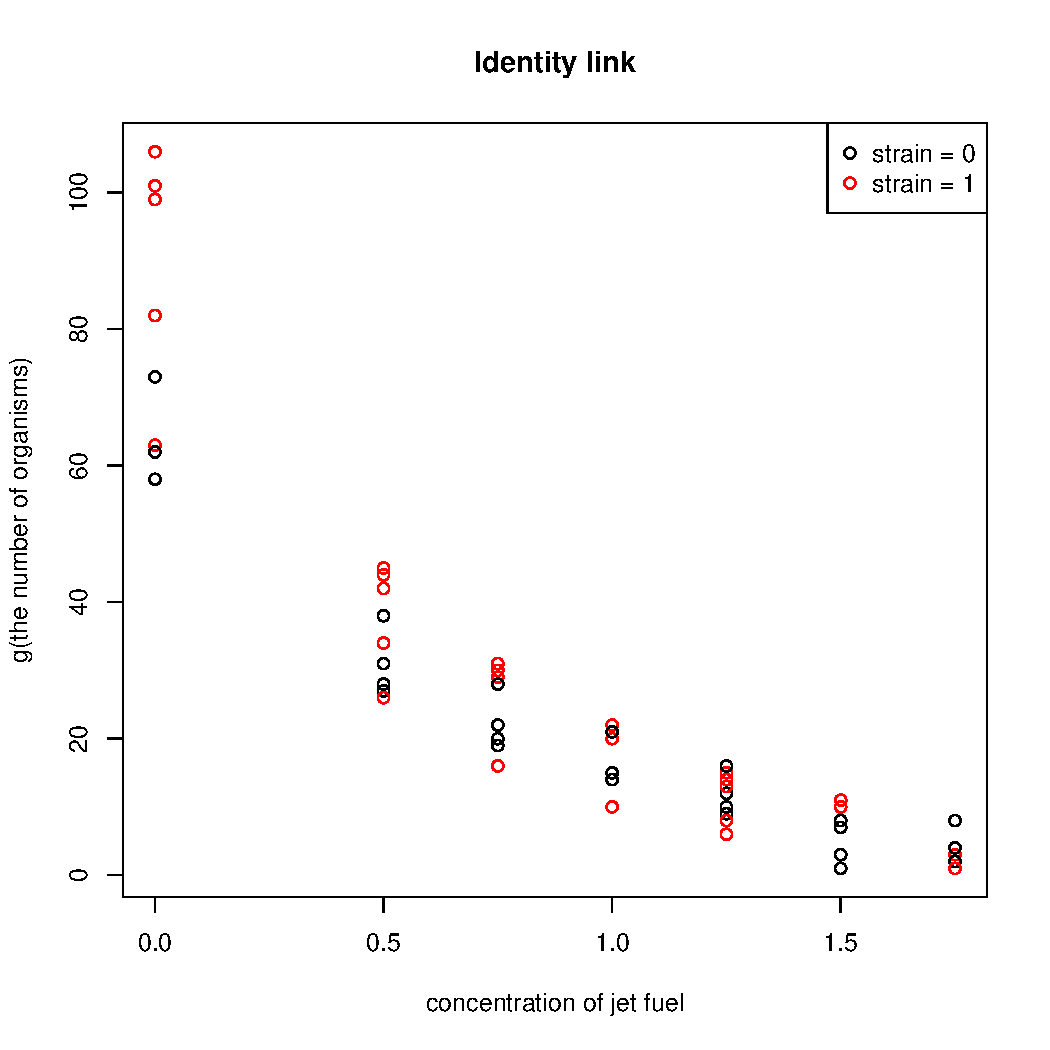
\includegraphics[width = \textwidth]{pic/HW2_4/Identity_link}
		\caption{"Identity link"}
		\label{Ide}
	\endminipage\hfill
	\minipage{0.5\textwidth}
		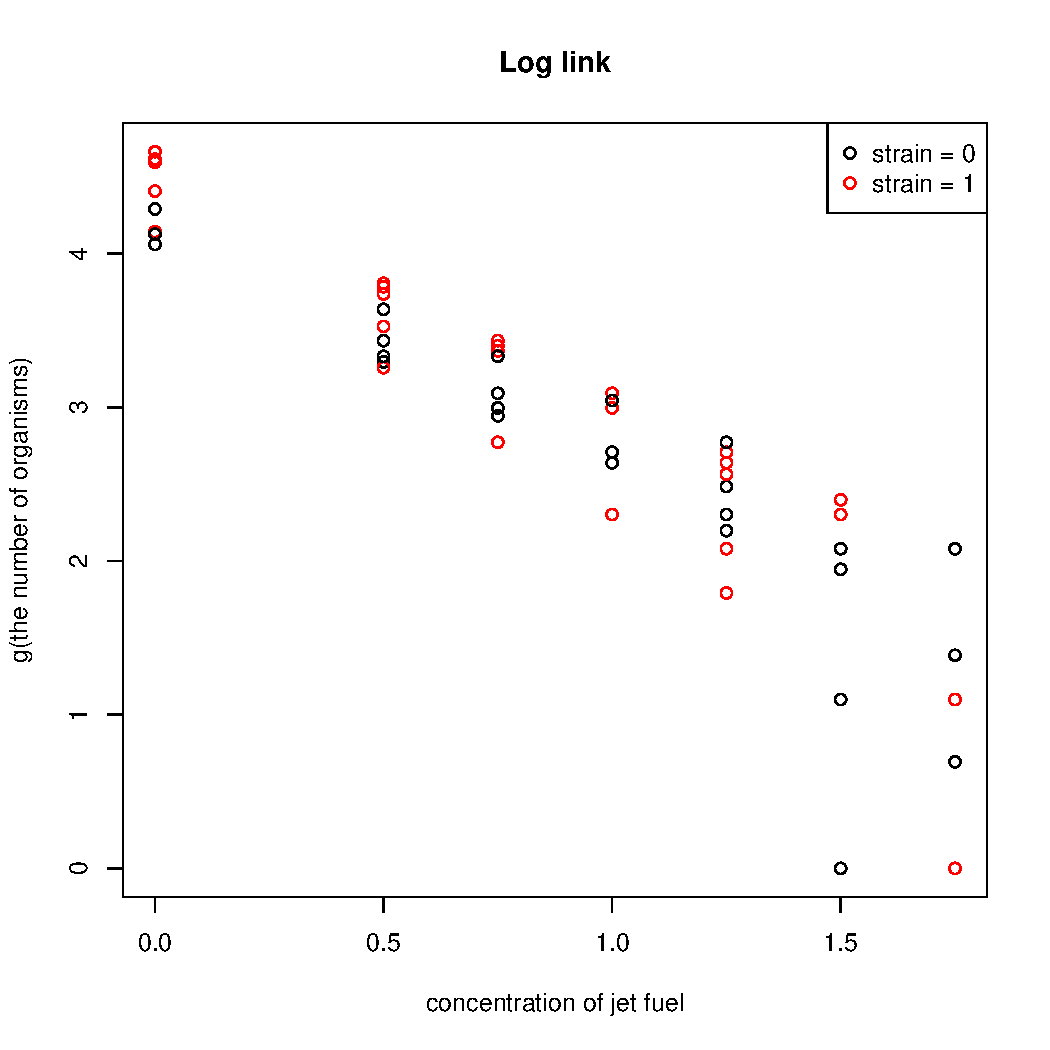
\includegraphics[width = \textwidth]{pic/HW2_4/Log_link}
		\caption{"Log link"}
		\label{Log}
	\endminipage\hfill
	\minipage{0.5\textwidth}
		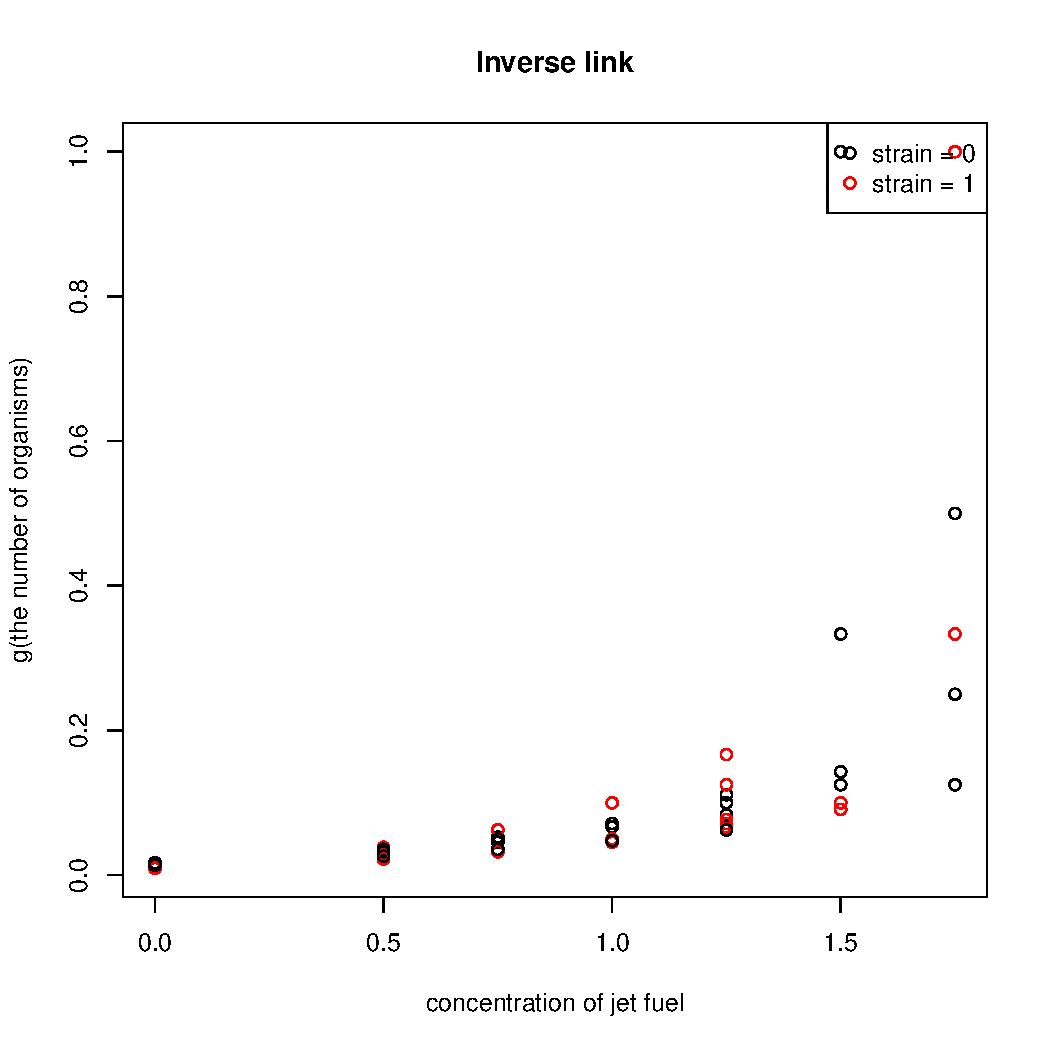
\includegraphics[width = \textwidth]{pic/HW2_4/Inverse_link}
		\caption{"Inverse link"}
		\label{Inv}
	\endminipage\hfill
	\minipage{0.5\textwidth}
		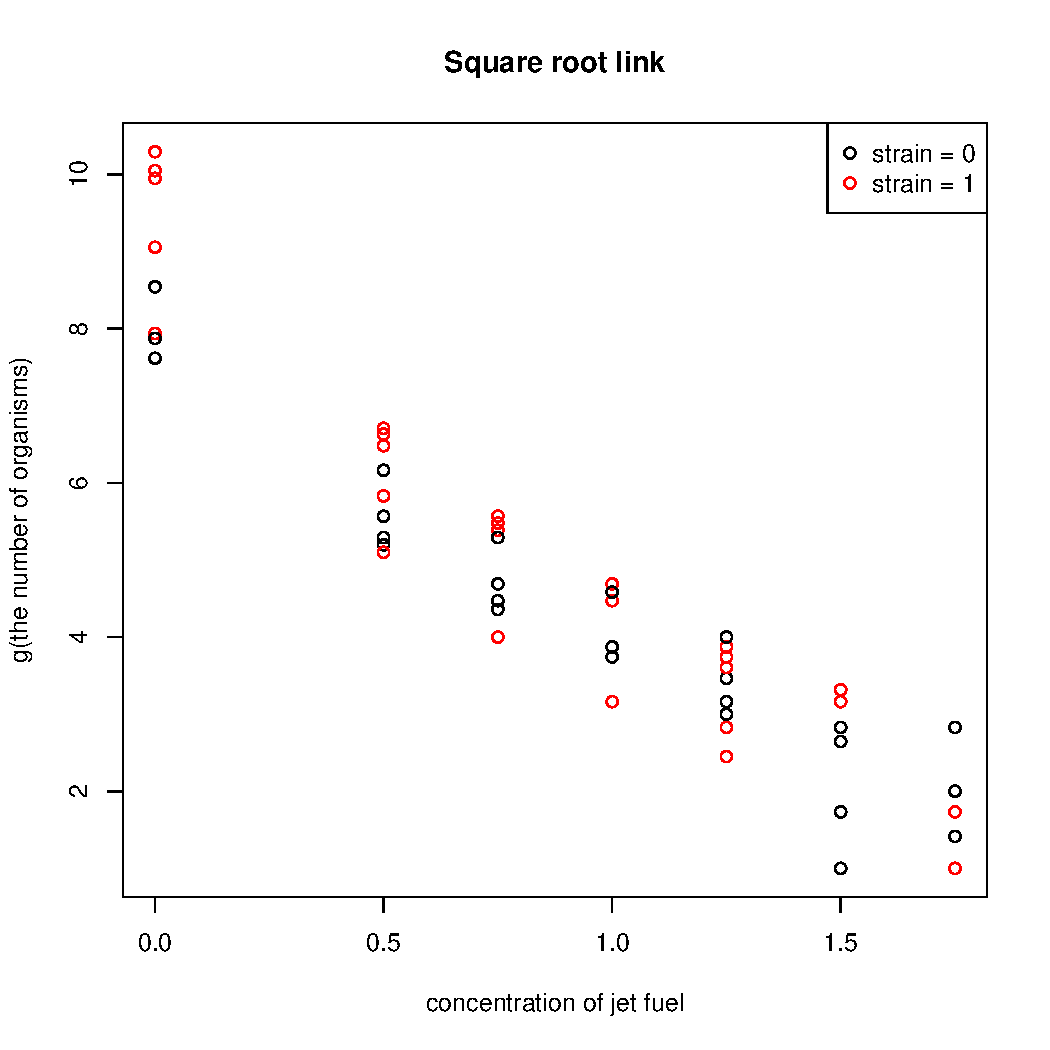
\includegraphics[width = \textwidth]{pic/HW2_4/Square_root_link}
		\caption{"Square root link"}
		\label{Squ}
	\endminipage\hfill
\end{figure}
\begin{table}
	\centering
	\caption{Different Poisson GLM with different link functions}
	\begin{tabular}{|c|c|c|c|}
		\hline
		& Deviance & AIC & BIC \\
		\hline
		Identity link & 291.84 & 621.42 & 622.35 \\
		\hline
		Log link & 86.38 & 415.95 & 416.88 \\
		\hline
		Inverse link  &165.04 & 494.62 & 495.55 \\
		\hline
		Square root link & 144.18 & 473.75 & 474.68 \\
		\hline
	\end{tabular}
	\label{glm}
\end{table}

\begin{figure}
	\centering
	\minipage[t]{0.25\textwidth}
	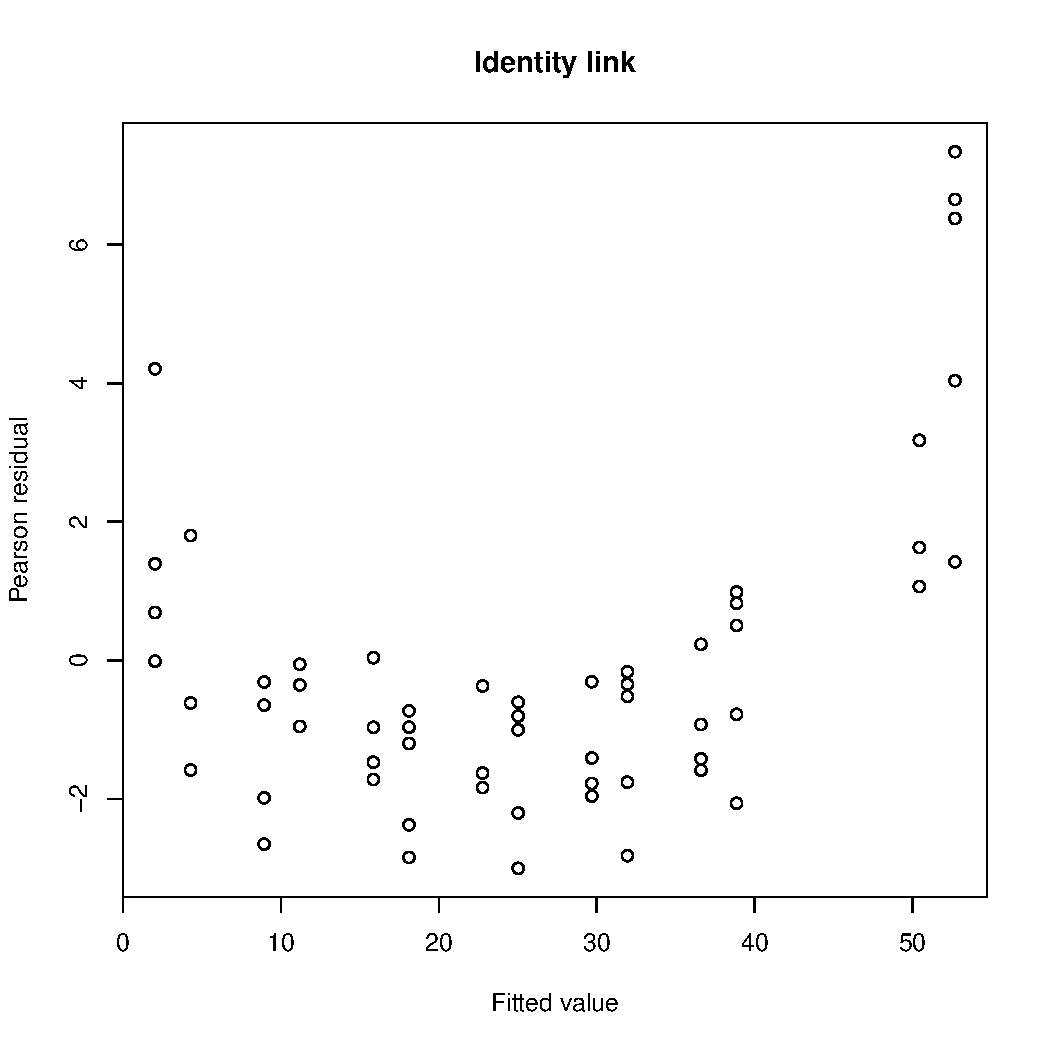
\includegraphics[width = \textwidth]{pic/HW2_4/p_res_ide}
	\caption{"Identity link"}
	\label{P_res_ide}
	\endminipage\hfill
	\minipage[t]{0.25\textwidth}
	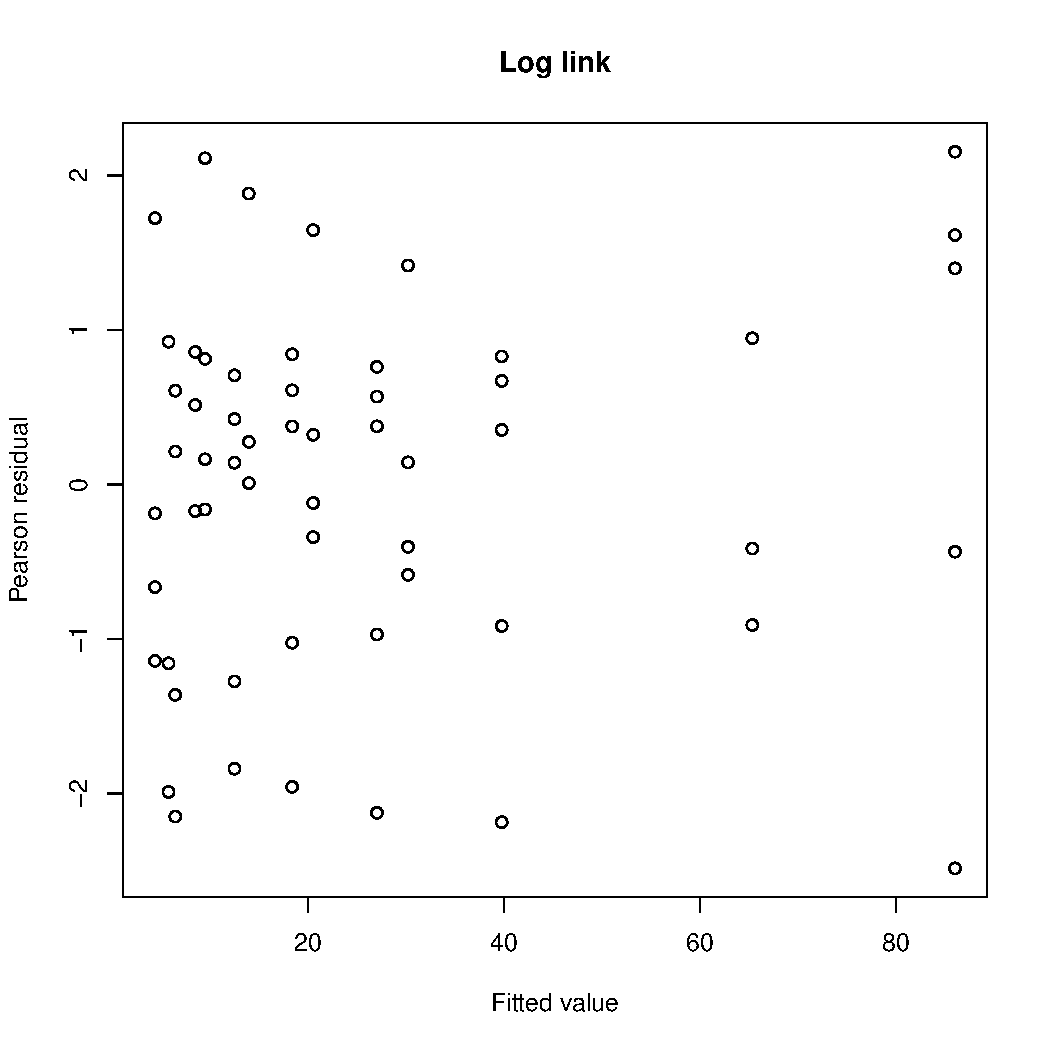
\includegraphics[width = \textwidth]{pic/HW2_4/p_res_log}
	\caption{"Log link"}
	\label{P_res_log}
	\endminipage\hfill
	\minipage[t]{0.25\textwidth}
	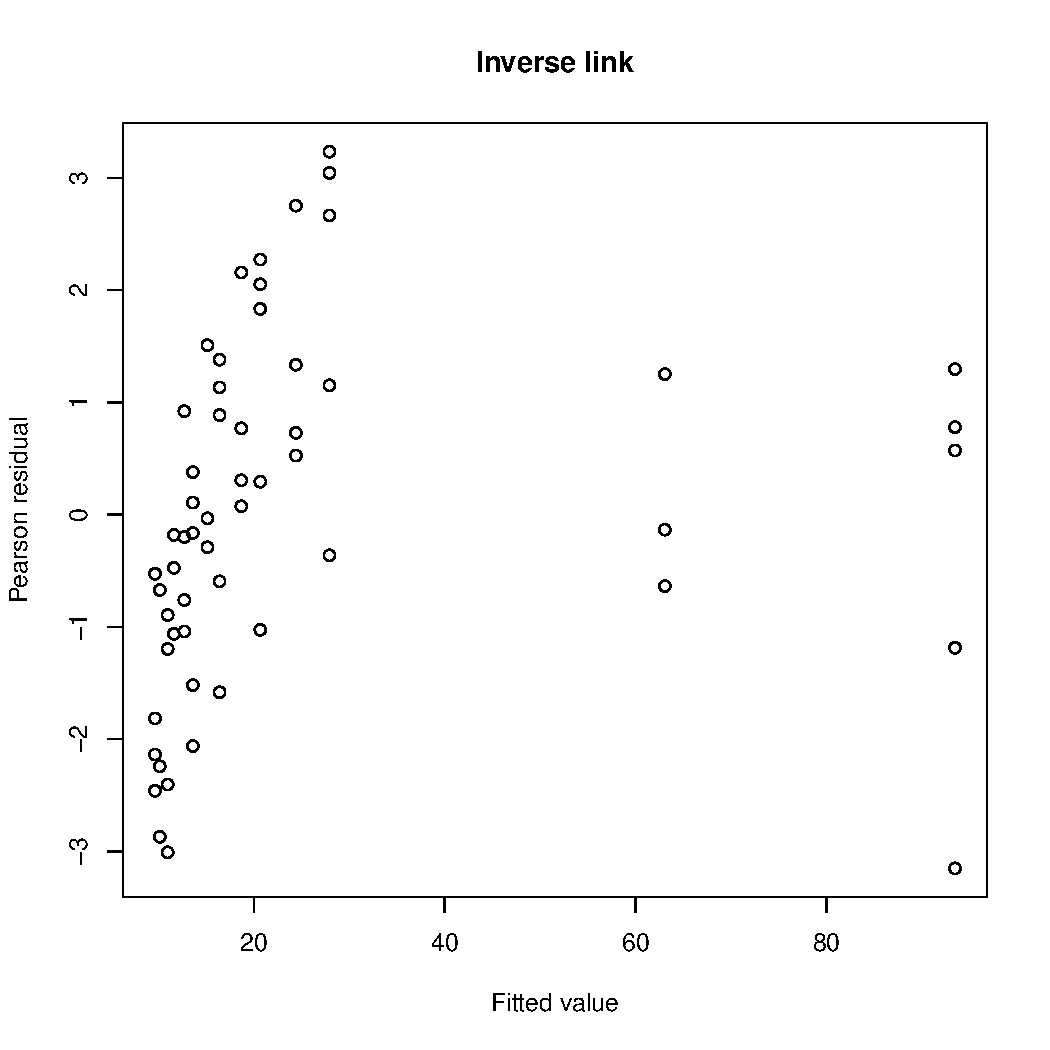
\includegraphics[width = \textwidth]{pic/HW2_4/p_res_inv}
	\caption{"Inverse link"}
	\label{P_res_inv}
	\endminipage\hfill
	\minipage[t]{0.25\textwidth}
	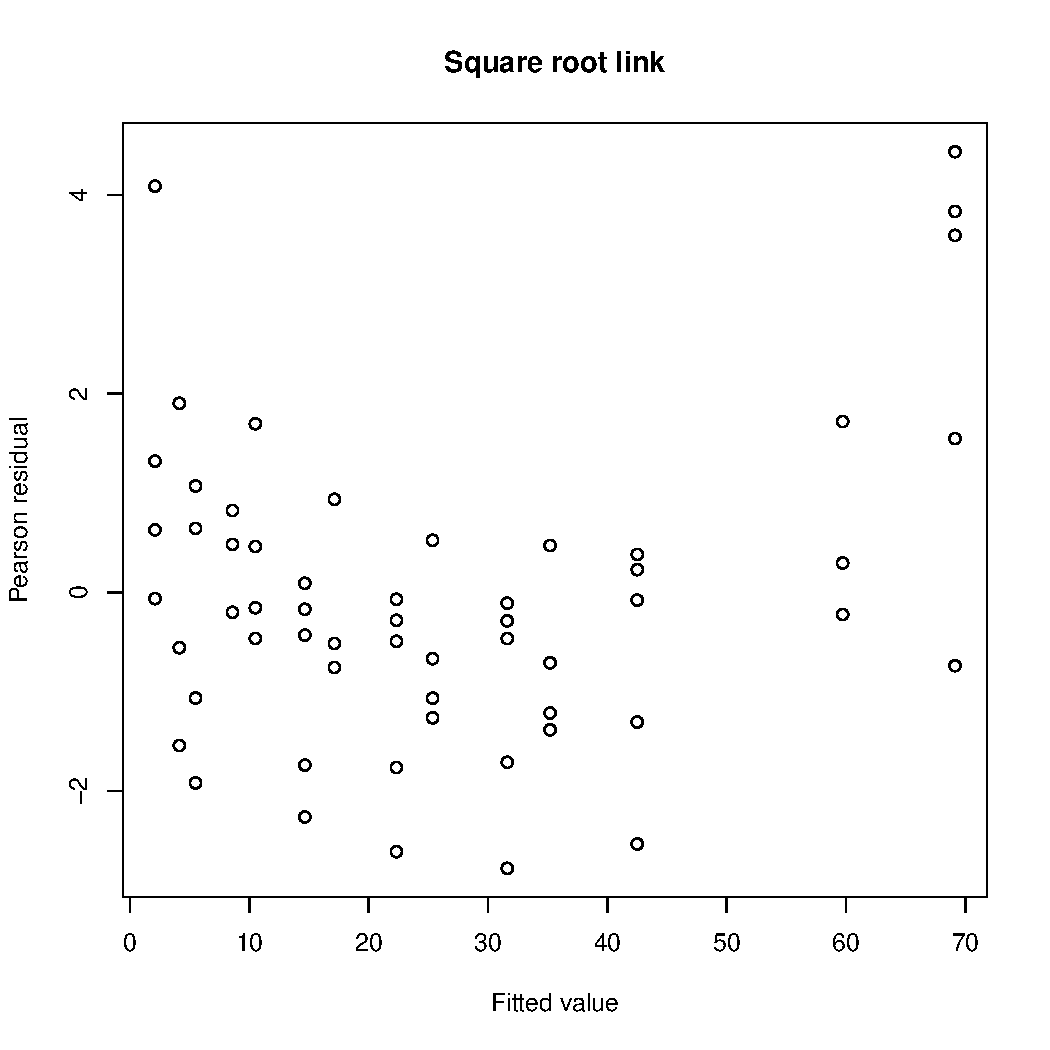
\includegraphics[width = \textwidth]{pic/HW2_4/p_res_squ}
	\caption{"Square root link"}
	\label{P_res_squ}
	\endminipage\hfill
	
	\minipage[t]{0.25\textwidth}
	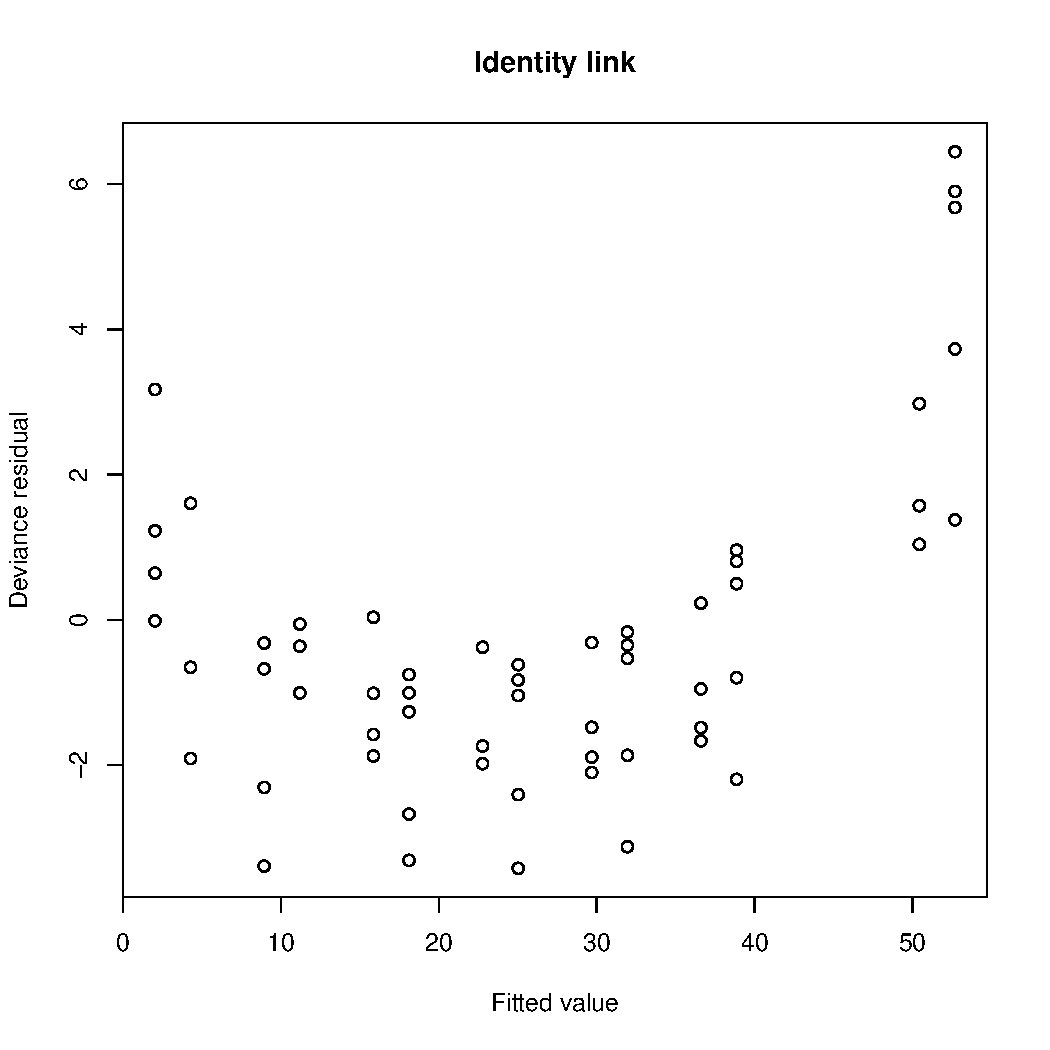
\includegraphics[width = \textwidth]{pic/HW2_4/d_res_ide}
	\caption{"Identity link"}
	\label{D_res_ide}
	\endminipage\hfill
	\minipage[t]{0.25\textwidth}
	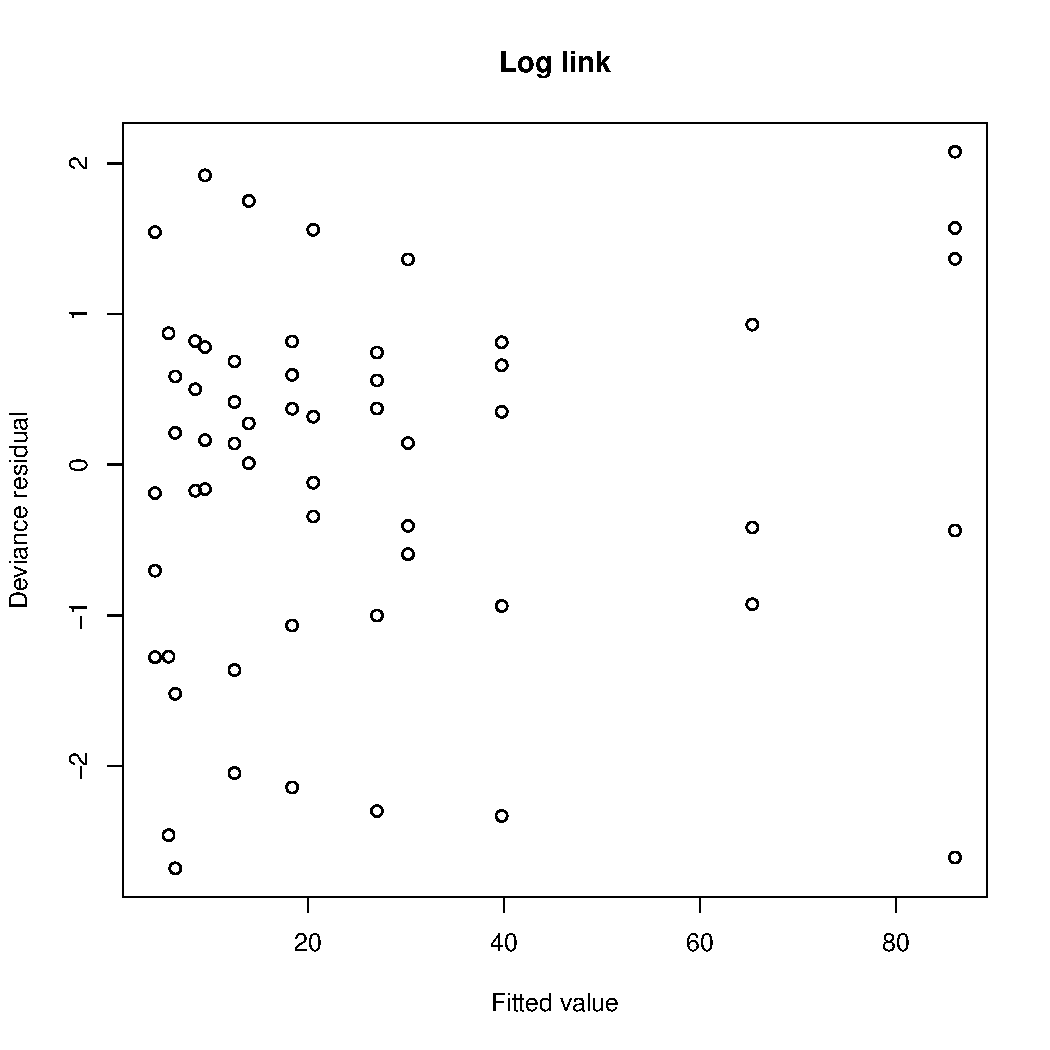
\includegraphics[width = \textwidth]{pic/HW2_4/d_res_log}
	\caption{"Log link"}
	\label{D_res_log}
	\endminipage\hfill
	\minipage[t]{0.25\textwidth}
	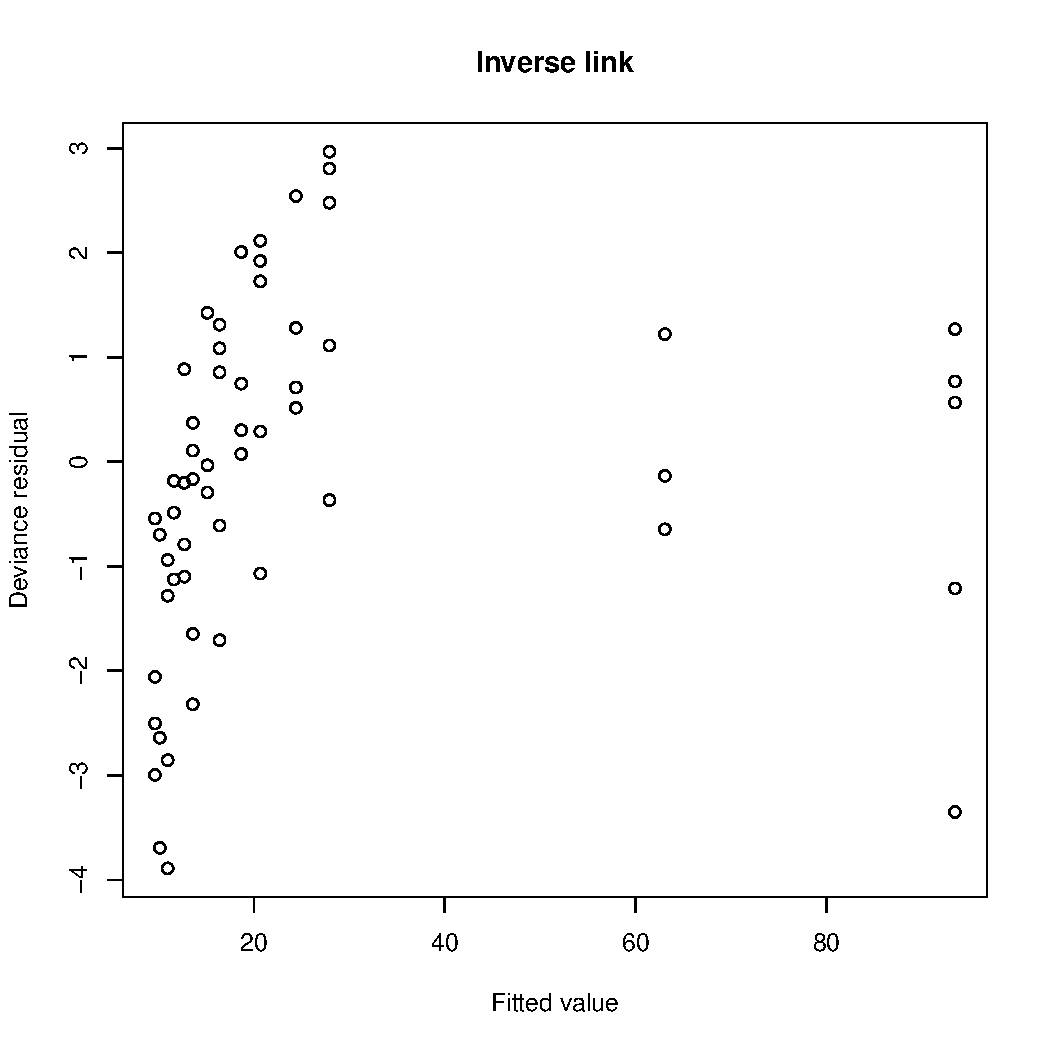
\includegraphics[width = \textwidth]{pic/HW2_4/d_res_inv}
	\caption{"Inverse link"}
	\label{D_res_inv}
	\endminipage\hfill
	\minipage[t]{0.25\textwidth}
	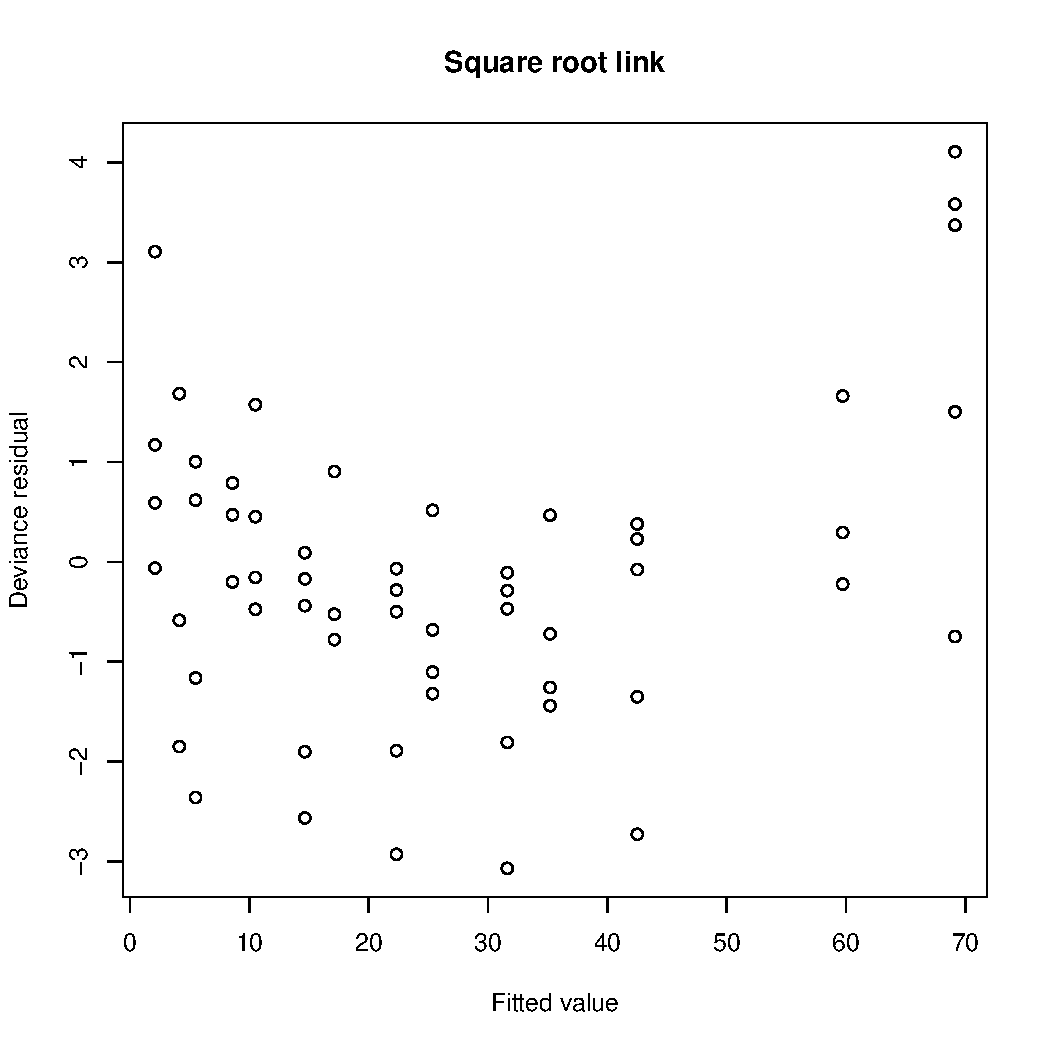
\includegraphics[width = \textwidth]{pic/HW2_4/d_res_squ}
	\caption{"Square root link"}
	\label{D_res_squ}
	\endminipage\hfill
\end{figure}

\begin{figure}
	\centering
	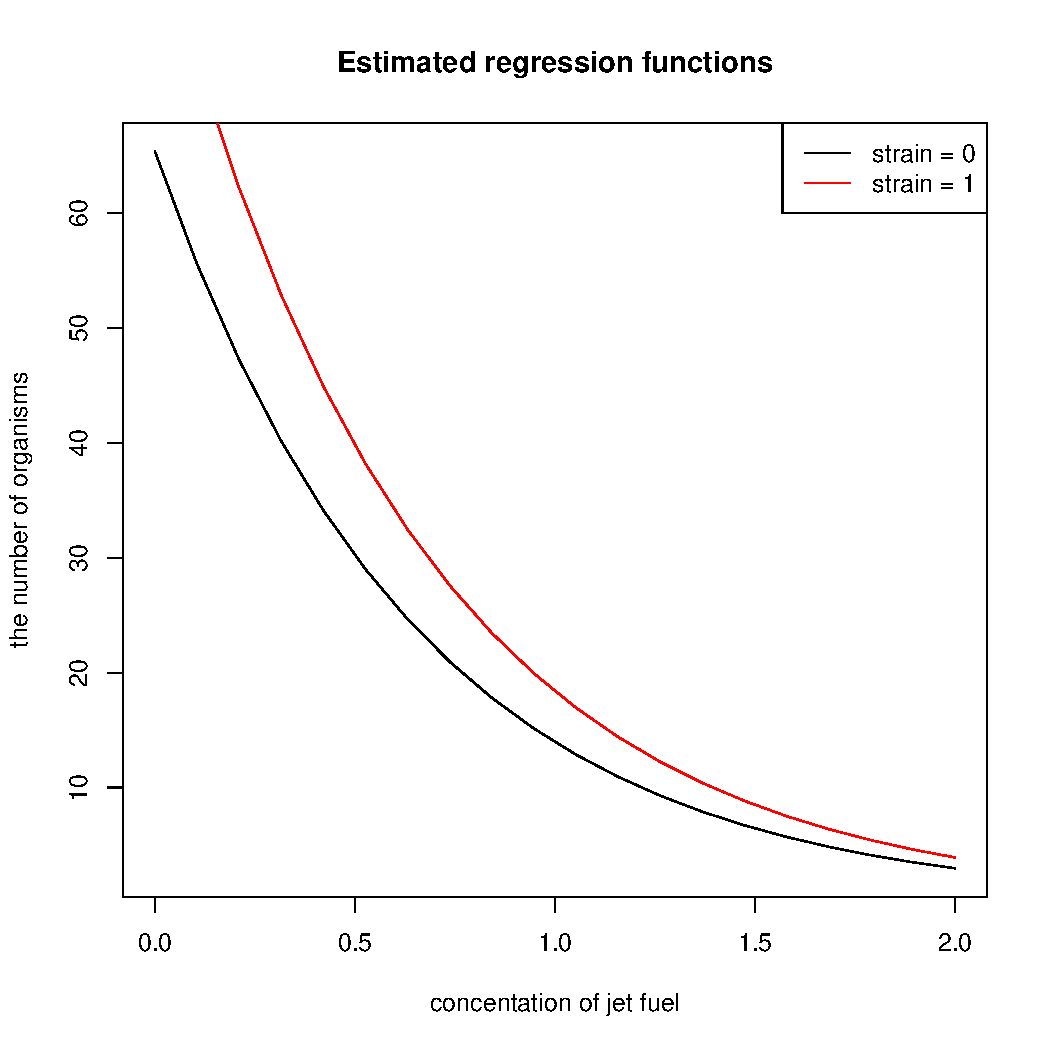
\includegraphics[width = \textwidth]{pic/HW2_4/est_func}
	\caption{Estimated regression functions}
	\label{est_func}
\end{figure}
}

\end{enumerate} 


\begin{thebibliography}{99}
%\bibitem{bost} Dennis D. Boos \& Leonard A. Stefanski (2013). \emph{Essential Statistical Inference}, Springer Texts in Statistics, Springer.
%\bibitem{pawi} Yudi Pawitan (2001). \emph{In All Likelihood}, Oxford University Press.
\end{thebibliography}

\end{document} 
